\chapter{Barnes-Hut algorithm}
The idea behind the Barnes-Hut algorithm differs substantially from previously described mesh-based methods.
The algorithm deals with gravitational forces directly instead of deriving them from the mesh-defined potential, as was the case with the PM and \PThreeM{} methods.
Significant reduction of time complexity, from quadratic to $O(N \log N)$, is achieved by approximating the potential due to ``far enough'' groups of particles by the initial terms of its multipole expansion \cite{trenti2008gravitationalnbodysimulations}.
The grouping of particles is hierarchical in nature and is thus best understood as a tree.
The entire set of particles comprises the top-level group, represented by the root of the tree;
the eight children of the root node are representative of groups of particles residing in each of the octants of the computational domain, etc.
The process of subdividing the space into eight smaller volumes at each node continues recursively until there is only one or zero particles left in a given volume.
Nodes that satisfy this condition are the leaves of the tree and are sometimes called the \textit{external nodes}.
The remaining nodes, each of which has eight children, are called \textit{internal nodes}.

In the basic variant of the algorithm, the potential due to a group of particles is approximated using only the monopole term with respect to the center of mass of the group, i.e.,
\begin{equation*}
    \phi_\text{mon}(r) = -\frac{GM}{r},
\end{equation*}
where $M$ is the group's total mass.
Since the potential is expanded about the center of mass, the dipole moment $\mathbf{p} = \sum_{i} m_i \mathbf{r}_i$ vanishes.
Hence, the next possible improvement comes from including the quadrupole term
\begin{equation*}
    \phi_\text{quad}(r) = -\frac{G}{2r^5} \mathbf{r} \cdot (\mathbf{Q} \mathbf{r}),
\end{equation*}
where $\mathbf{Q}$ is the quadrupole moment tensor defined as
\begin{equation*}
    Q_{ij} = \sum_{k} (3r_{ki}r_{kj} - 3r_k^2\delta_{ij})m_k.
\end{equation*}
In theory, we could keep on adding more terms to improve the quality of the approximation.
In our implementation, however, we restrict ourselves to the quadrupole term.

\section{Building the tree} % checked
The data structure that fits the description given in the introduction is called an \textit{octree}.
An internal node of the octree stores the COM vector, the total mass of the group it represents, and the quadrupole tensor, whereas an external node stores a reference to the actual particles (or is empty if no particle was found in its associated volume).
The recursive procedure of building the tree is shown in \autoref{alg:bh-tree-insert}.
\begin{algorithm}
    \caption{Insert a particle into the Barnes-Hut tree}\label{alg:bh-tree-insert}
    \begin{algorithmic}[1]
        \Function{Insert}{$n$, $p$}
        \If{$n$ is an internal node}
        \State Update $n.\textrm{COM}$ and total mass $n.M$ of $n$ with $p$
        \State \Call{Insert}{child of $n$ that should contain $p$, $p$}
        \ElsIf{$n$ is empty}
        \State Assign $p$ to $n$
        \Else \Comment{Occupied external node}
        \State Subdivide $n$ into child nodes
        \State Move existing particle $p'$ in $n$ into child that should contain $p'$
        \State Update center of mass and total mass of $n$ with $p$ and $p'$
        \State \Call{Insert}{child of $n$ that should contain $p$, $p$}
        \EndIf
        \EndFunction
    \end{algorithmic}
\end{algorithm}
The quadrupole moment tensor for each node is calculated once the whole tree is already built.
The recursive relation used in this calculation is given in \cite{hernquist1987performance} and reads
\begin{equation*}
    \mathbf{Q} = \sum_{\text{child }c} \mathbf{Q}_c + \sum_{\text{child }c} m_c(3 \mathbf{R}_c \otimes \mathbf{R}_c - R_c^2 \mathbf{I}),
\end{equation*}
where $\mathbf{R}_c = \mathbf{x}^\text{COM}_c - \mathbf{x}^\text{COM}$ is the displacement vector from the COM of child $c$ to the COM of the parent, $\mathbf{I}$ is the identity matrix, and $\otimes$ denotes the outer product.

For reasons that will become apparent later, it can be beneficial to separate the COM calculation from the tree creation part.
In such a case, the COM is calculated recursively using the relation
\begin{equation}\label{eq:bh-com-calculation}
    \mathbf{x}^\text{COM} = \frac{\sum_{\text{child } c} m_c \mathbf{x}_c^\text{COM}}{\sum_{\text{child } c} m_c}
\end{equation}
after the tree has already been built (and obviously before the quadrupole moment calculation).

\section{Acceleration calculation}
In the Barnes-Hut algorithm, the net acceleration of a particle $p$ is calculated by summing the contributions from single particles or groups of particles while traversing the tree.
The decision whether the acceleration can be approximated using the information stored in an internal node $n$ depends on the relative distance from $p$ to $n.\textrm{COM}$ (the center of mass of group represented by $n$).
The distance is relative to the \textit{width} $H$ of the node, i.e. the side length of the cubical volume encompassed by the node.
More concretely, the approximation takes place if $n.H / |n.\mathrm{COM} - p.\mathbf{x}| < \theta$, where $\theta$ is the so-called \textit{opening angle}.
In the extreme case when $\theta$ is set to zero, no approximations take place, and the algorithm reduces to the PP method.
The procedure described above is illustrated in \autoref{alg:bh-find-force}.
\begin{algorithm}
    \caption{Compute gravitational force on a particle using Barnes-Hut approximation}
    \label{alg:bh-find-force}
    \begin{algorithmic}[1]
        \Function{FindAcceleration}{$n$, $p$, $\theta$}
        \If{$n$ is an external node}
        \If{$n$ contains a particle $q \neq p$}
        \State $p.\mathbf{a} \gets p.\mathbf{a} + \Call{GravitySoft}{q.\mathbf{x}, q.m, p.\mathbf{x}} / p.\text{mass}$
        \EndIf
        \State \Return
        \EndIf
        \If{$n.H / |n.\text{COM} - p.\mathbf{x}| < \theta$}
        \State $p.\mathbf{a} \gets p.\mathbf{a} + \Call{Gravity}{n.\mathrm{COM}, n.M, p.\mathbf{x}}$
        \State \Return
        \EndIf
        \ForAll{child $n_c$ of $n$}
        \State \Call{FindAcceleration}{$n_c$, $p$, $\theta$}
        \EndFor
        \EndFunction
    \end{algorithmic}
\end{algorithm}
In the implementation, the \textsc{GravitySoft} function calculates the gravitational force softened by $\epsilon$, i.e. it returns the value given by \autoref{eq:softened-force}.
The pairwise potential energy associated with this force is given by
\begin{equation}\label{eq:pe-soft}
    \Phi_{ij}^\textrm{soft} = - \frac{G m_i m_j}{\sqrt{r_{ij}^2 + \epsilon^2}}.
\end{equation}
The \textsc{Gravity} function returns the approximation (up to the quadrupole term) of the acceleration due to a group of particles represented by a given node, i.e.
\begin{equation*}
    \mathbf{a} = -GM \frac{\mathbf{r}}{r^3} + \frac{G}{r^5}\mathbf{Q}\mathbf{r} - \frac{5G}{2}(\mathbf{r} \cdot (\mathbf{Q} \mathbf{r})) \frac{\mathbf{r}}{r^7}
\end{equation*}
(see \cite{hernquist1987performance}).

One possible way to quantify the quality of approximation for a given value of $\theta$ is to consider the relative error of calculated force.
We set the same initial conditions of the system for both the PP direct summation method and the Barnes-Hut algorithm, compute the deviation of Barnes-Hut forces from PP forces acting on each particle, and take the average over all particles.
In other words, the error calculated is given by the \autoref{eq:force-avg-relative-err}.
The dependence of the error on the opening angle $\theta$ and the corresponding execution time are shown in \autoref{fig:bh-analysis}.
The figure includes plots for two cases: when only the monopole term is used in the Barnes-Hut approximation, and when both the monopole and quadrupole terms are included.
As can be seen, the quadrupole-based algorithm exhibits significantly improved error scaling with increasing $\theta$.
Naturally, this raises the question of the additional computational cost incurred by the inclusion of the quadrupole term.
Our tests showed that this impact is minimal.
The results (for $N = 10{,}000$ particles and $0 \leq \theta \leq 2$) support this observation.
\begin{figure}[htp]
    \centering
    \begin{subfigure}[b]{0.47\textwidth}
        \centering
        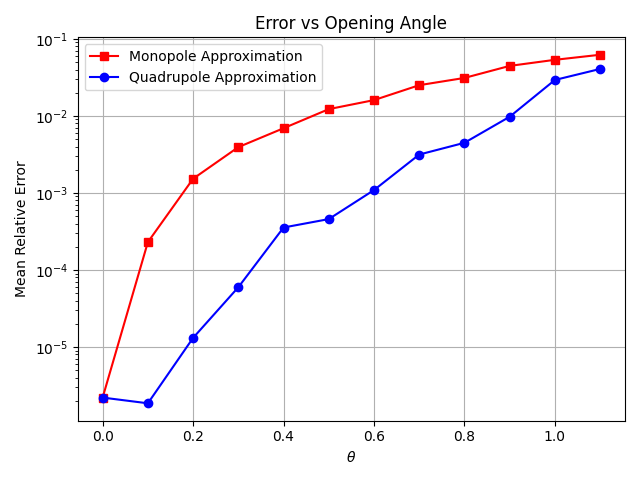
\includegraphics[width=\textwidth]{chapters/barnes-hut/img/error-vs-theta.png}
        \caption{Force approximation error.}
        \label{fig:bh-force-error}
    \end{subfigure}
    \hfill
    \begin{subfigure}[b]{0.47\textwidth}
        \centering
        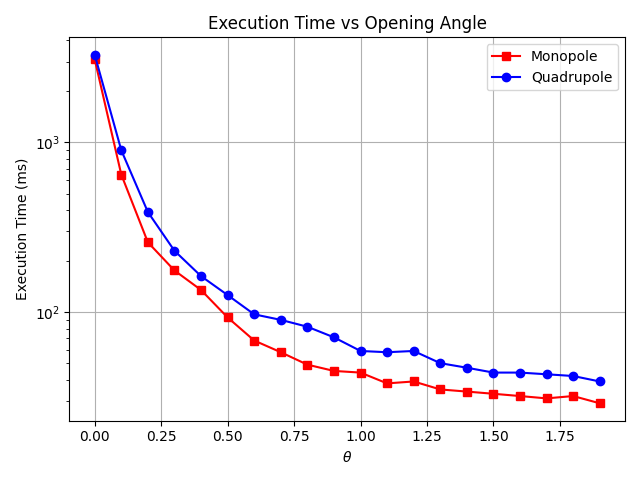
\includegraphics[width=\textwidth]{chapters/barnes-hut/img/bh-time.png}
        \caption{Execution time per iteration.}
        \label{fig:bh-time}
    \end{subfigure}
    \caption{Comparison of error and execution time in the Barnes-Hut algorithm using monopole and quadrupole approximations.}
    \label{fig:bh-analysis}
\end{figure}
Both tests described above were conducted on a uniform disk particle distribution.

We note that direct calculation of total potential energy is infeasible as $O(N^2)$ operations would be required.
Instead, we use an approximation based on the values stored in the tree.
The approximate value of the potential energy is accumulated for each particle using a procedure analogous to force calculation.
Indeed, the only difference between the two is the replacement of gravitational force calculation in \autoref{alg:bh-find-force} with potential energy calculation according to \autoref{eq:pe-soft}.

It is also noteworthy that the procedure outlined in \autoref{alg:bh-find-force} is embarrassingly parallel.
In our CPU implementation, the workload is split between an arbitrary number of threads on particle-by-particle basis.

\section{Accelerating tree construction}\label{sec:accelerating-tree-construction}
Unlike the force calculation part which is easily parallelized, the tree construction step is inherently sequential.
An approach to parallel tree construction outlined in \cite{warren_salmon_1993} involves splitting the set of particles into load-balanced spatial groups which are then used to construct separate trees (one per thread), with the final step being the merge of the created trees.
The merge step is highly involved and beyond the intended scope of this thesis.
For this reason, we propose an alternative approach to accelerating the tree construction which does not involve building the tree in parallel.

Our strategy, based on the ideas put forth in \cite{warren_salmon_1993}, stems from an observation that a potential bottleneck in \autoref{alg:bh-tree-insert} is related to irregular accesses to the nodes of the tree.
Inserting two particles separated by a large spatial distance leads to visiting nodes along two completely different paths in the tree which results in a huge number of cache misses.
A solution to this problem is to sort the list of particles in such a way that subsequent particles on the list (typically) lie close to each other in the physical space.
An ordering with this property can be generated by numbering the particles based on their position along a chosen \textit{space-filling curve}.

A space filling curve can be thought of as the limit of an infinite sequence of curves which ``fill'' the space without ``holes'' \cite{WeissteinPlaneFilling}.
In the limit, the curve reaches every point of the space, but due to practical constraints we can only deal with an approximation, i.e. some member of the limiting sequence.
In our implementation, we are working with a \textit{Z-order curve}, also called a \textit{Morton space-filling curve}, so it will in the focus of our discussion.
To make the visualization simpler, assume that the computational domain is two-dimensional and coarsely divided into 16 cells (particles within the same cells are ordered arbitrarily).
Then, the Z-order curve that covers all 16 cells is shown in \autoref{fig:z-order-curve}.
\begin{figure}[htp]
    \centering
    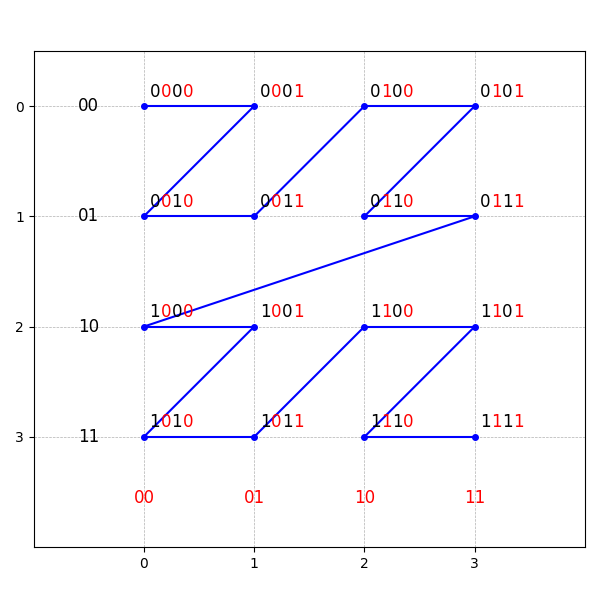
\includegraphics[scale=0.5]{chapters/barnes-hut/img/z-order.png}
    \caption{Z-order curve.}
    \label{fig:z-order-curve}
\end{figure}
The ordering of the points along the curve is obtained by assigning each cell a \textit{Z-value}, whose binary representation is calculated by interleaving the bits of the $x$ and $y$ coordinates.
This is illustrated in \autoref{fig:z-order-curve} by coloring the $x$- and $y$-coordinate bits red and black respectively.

In a standard setting, the coordinates of a particle are given by real numbers and not integers however.
In order to establish a mapping between the two, we have to first decide on the intended resolution of the grid.
In our implementation, we use the 32-bit integer type to represent the Z-values, which means that each coordinate should be represented by a 10-bit integer number ($3 \times 10 = 30 \leq 32$).
Thus, the mapping from real-valued coordinate of a particle to an integer one is given by
\begin{equation*}
    \left\lfloor \frac{(x - \text{low}.x)}{H} \times (2^{10} - 1)\right\rfloor \in [0, 2^{10}),
\end{equation*}
where $\text{low}$ and $H$ define the computational domain as
\begin{equation*}
    \text{domain} = [\text{low}.x, \text{low}.x + H] \times [\text{low}.y, \text{low}.y + H] \times [\text{low}.z, \text{low}.z + H].
\end{equation*}

In our proposed optimization, we make the following changes into the tree construction algorithm (\autoref{alg:bh-tree-insert}):
\begin{enumerate}
    \item The insertion does no longer start at the root of the tree for each particle but at the last inserted to node,
    \item The COM calculation is deferred until the tree construction is finished and carried out using \autoref{eq:bh-com-calculation}.
\end{enumerate}
The second point is a direct consequence of the first one;
if the insertion of a particle does not start at the root but at some other node $n$, deep in the tree, the nodes lying above $n$ will not be updated so their COM and total mass values will be incorrect.
The first point, however, requires more explanation.
Since the particles are z-ordered, subsequent inserts into the tree will result in traversing similar paths.
Because of that, the point of insertion can be found more efficiently by starting the traversal from the last seen node and backtracking up the tree until a valid insertion point is found.
The decision whether to stop backtracking at a given node $n$ is made on the condition that the particle to be inserted is inside a cube represented by $n$.
When the condition is met, the standard insertion procedure takes place starting at $n$.

The asymptotic time complexity of the modified tree construction algorithm is the same as for the standard one.
Sorting the particles requires $O(N\log N)$ operations but inserting a particle into the tree starting at the last-seen node is an $O(1)$ operation.
The last claim may raise objections, since some number of backtrack steps is expected on each insert.
To verify it, we measured the average number of backtracks per particle in typical simulations and found that it did not exceed $2.5$ (this can be compared with the number of backtracks required when the particles are not z-ordered; in such a case, we found that in the tested scenarios, on average more than 8 backtracks were typically needed).
Even though the modified algorithm still has the $O(N\log N)$ time complexity, it leads to more predictable memory access patterns which results in noticeably improved performance.
The tree construction time as a function of $N$ is shown in \autoref{fig:z-order-tree-time}.
\begin{figure}[htp]
    \centering
    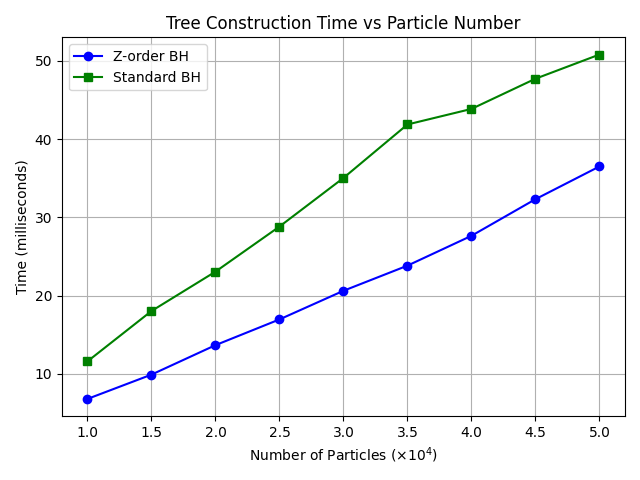
\includegraphics[scale=0.5]{chapters/barnes-hut/img/tree_construction_time.png}
    \caption{Tree construction time averaged over the number iterations of the simulation ($\theta = 1$).}
    \label{fig:z-order-tree-time}
\end{figure}
For the purposes of generating the graphs shown there, the tree construction time was measured in a spiral galaxy simulation.
As can be seen in the figure, the improved algorithm allows for up to $40\%$ speedup over the standard version.
In our tests, we used the standard library procedure \texttt{std::sort} with the parallel execution policy, which offered a slight speedup over the sequential variant.
